
%\documentclass[12pt]{report}
%\documentclass[12pt]{extreport}
\documentclass[17pt]{extarticle}
%\documentclass{memoir}

\usepackage{graphicx}
\usepackage{setspace}
\usepackage{amsmath,amssymb}
\usepackage{IEEEtrantools}
\usepackage{cancel}
\usepackage[font=small,labelfont=bf]{caption}


\usepackage{verbatim}

\usepackage[T1]{fontenc}
\usepackage[utf8]{inputenc}
\usepackage[italian]{babel}

%\usepackage{hyperref}


%\usepackage{imakeidx}%
%\makeindex[program=xindy]%, options=-C utf8 -L portuguese]%
%\usepackage{makeidx}
%\makeindex

\usepackage{imakeidx}
\usepackage{hyperref}
\makeindex


\usepackage{geometry}
 \geometry{
 a4paper,
 total={170mm,264mm},
 left=2mm,
 top=10mm,
 }

\begin{document}

%\backmatter
%text\index{test}
%\printindex


\begin{flushright}
{\bf \today}
\end{flushright}

\tableofcontents

\clearpage


Abbiamo visto analiticamente\footnote{Cioè facendo i calcoli} che, data una equazione lineare in due incognite $x$ e $y$, una sua possibile soluzione è una \emph{coppia ordinata} di numeri. 


Ad esempio, data l'equazione 

\begin{equation}\label{eq:eqLineare}
	9y - 7x - 3 = 0
\end{equation}

attribuendo a $x$ il valore $0$, si ottiene per $y$ il valore $\frac{1}{3}$, attribuendo a $x$ il valore $1$, si ottiene per $y$ il valore $\frac{10}{9}$ e così via, come nella tabella che segue


\begin{center}
\begin{tabular}%\label{tab:eqLineare}
	{ |c|c| c| }
 \hline
 {\bf x} &  {\bf y} &  $y$ approssimato \\ 
 \hline
 0 & $\frac{1}{3}$  &  $0,33$ \\
 1 & $\frac{10}{9}$ &  $0,11$ \\ 
 2 & $\frac{17}{9}$ &  $1,89$ \\ 
 3 & $\frac{24}{9}$ &  $2,67$ \\ 
 4 & $\frac{31}{9}$ &  $3,44$ \\ 
 5 & $\frac{38}{9}$ &  $4,22$ \\ 
$\dots$ & $\dots$	& $\dots$\\	
 \hline

%\caption{Tabella delle possibile coppie ordinate di valori $x$ e $y$ soluzioni dell'equazione lineare in due incognite.}
\end{tabular}
\end{center}


essendo \emph{infiniti} i differenti valori che posso attribuire a $x$, infinite sono anche i possibili valori di $y$. Quindi, data una equazione lineare in due incognite, {\bf infinite sono le coppie ordinate di valori $x$ e $y$ che la soddisfano}.

Abbiamo anche visto, adoperando la carta millimetrata, che le infinite coppie ordinate che risolvono una equazione lineare come la eq. \ref{eq:eqLineare} \emph{giacciono tutte e solo} su una ben precisa retta. %Si dice, a tal proposito, di \emph{equazione della retta}.

Sempre adoperando la carta millimetrata, abbiamo visto che mettendo a sistema due differenti equazioni lineari, la coppia ordinata risultato del sistema è, graficamente, il punto di intersezione delle rispettive rette. In questa sede andiamo a rivedere tutto questo facendo uso del \emph{foglio di calcolo elettronico} e, in particolare, di LibreOffice Calc.

\section{Rappresentazione grafica di una retta su piano cartesiano con \emph{foglio di calcolo elettronico} }


%Inoltre, il risultato di un sistema due equazioni lineari e due incognite, quando ammette una unica soluzione\footnote{le soluzioni possono essere \emph{infinite} quando il sistema è indeterminato o nessuna, quando il sistema è \emph{impossibile}.}, è una \emph{coppia ordinata} di numeri che corrispondono alle coordinate del punto di intersezione tra le due rette associate a ciascuna delle due equazioni.

%Data una equazione lineare in due variabili $x$ e $y$, come ad esempio

%usiamo il foglio di calcolo elettronico e, in particolare, \emph{LibreOffice Calc}, per calcolare il valore delle coppie ordinate che soddisfano una equazione

%sono infinite
Prendiamo in considerazione il sistema due equazioni lineari e due incognite di pag 494 n 114 che riportiamo anche qui di seguito per comodità:

\begin{equation}\label{eq:sistema}
  	\begin{cases}
		\frac{x}{3} - \frac{3}{2}y = 2\\
		9y - 7x - 3 = 0		
	\end{cases}
\end{equation}

Facendo uso di LibreOffice Calc, per ciascuna delle equazioni di questo sistema, andiamo a calcolare una tabella, come quella del paragrafo precedente.

Per fare ciò, conviene che per ciascuna delle due equazioni del sistema \ref{eq:sistema}, esplicitiamo la $y$ in funzione della $x$


\begin{equation}\nonumber
  	\begin{cases}
		y = \frac{2}{9}x - \frac{4}{3}\\
		y = -\frac{7}{9}x - \frac{1}{3}
	\end{cases}
\end{equation}


Passiamo ora a LibreOffice Calc (fig. \ref{fig:LibreOfficeCalc000})
\begin{figure}[h!]		
	\centering
   	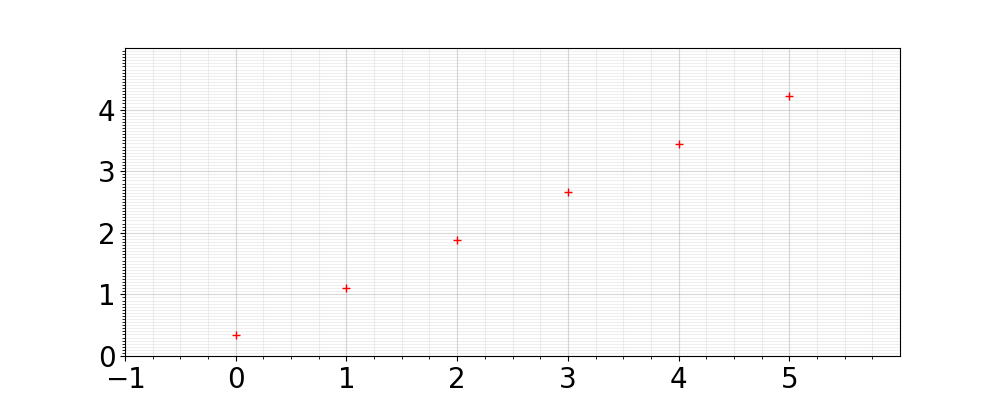
\includegraphics[width=8.0in]{pictures/picture_000.png}
  	\caption{Software}
   	\label{fig:graficoST_unAcce}
\end{figure}

e iniziamo a riempire la colonna dei valori di $x$, che useremo sia per calcolare i valori di $y$ della prima equazione ($y1$), sia per calcolare i valori di $y$ della seconda equazione ($y2$).


%Dobbiamo simulare la carta millimetrata, quindi consideriamo un intervallo delle x che vada da $-10$ a $+10$.

Anzichè partire dal valore $x = 0$, partiamo dal valore $x = -10$. Inoltre, Adoperiamo la \emph{colonna A} per scrivere i diversi valori di $x$ e, di questa, adoperiamo la riga 1 come \emph{indice di colonna} (fig. \ref{fig:LibreOfficeCalc001}.


\begin{figure}[h!]		
	\centering
   	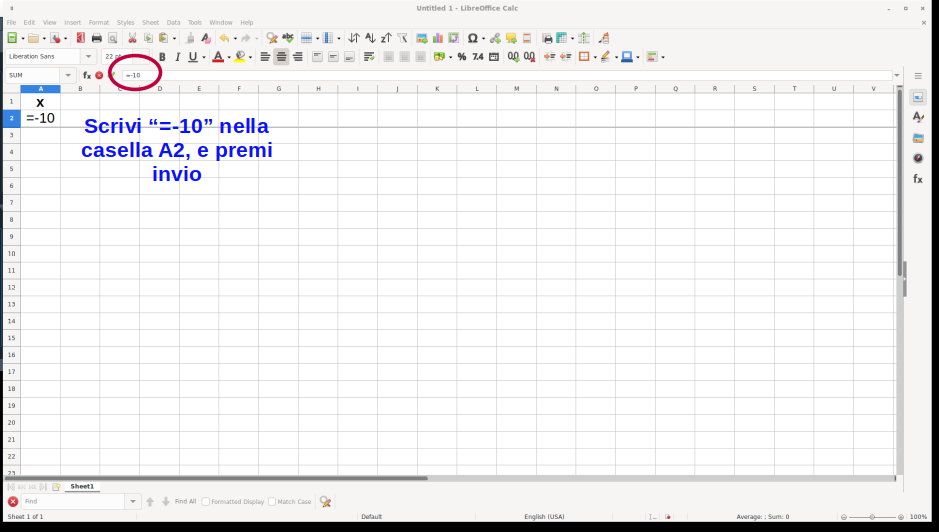
\includegraphics[width=8.0in]{pictures/picture_001.png}
   	\caption{LibreOffice Calc}
   	\label{fig:LibreOfficeCalc001}
\end{figure}



\end{document}